%---------- Inleiding ---------------------------------------------------------

\section{Introductie} % The \section*{} command stops section numbering
\label{sec:introductie}
Het idee achter Remote Procedure Calls gaat terug tot rfc707 uit 1976. rfc707 was een primitief RPC systeem dat beschreef hoe men in een gedistribueerd systeem al dan niet gelijktijdig bepaalde procedures laat uitvoeren. Vandaag de dag bestaan er verschillende implementaties van het RPC framework met elk hun eigen voor- en nadelen. Deze thesis focust zich op het door Google in 2016 uitgebrachte gRPC. Het gRPC heeft dan ook een server nodig om op te draaien. Bij het kiezen van een server taal zijn er vandaag de dag verschillende opties zoals Node, Java, PHP, Python en nog veel meer. Omdat gRPC redelijk jong is en betekent dat ook dat er nog geen beste taal is. De uitvoering van een snelheid vergelijkend onderzoek is niet voor elk bedrijf even financieel haalbaar. \\ \\ Het hoofddoel van dit onderzoek is het vergelijken en bespreken van het verschil in performantie tussen Node en .Net. De performantie zal aan de hand van generieke statistieken, zoals tijd en processorverbruik,  achterhaald worden. Ook zullen enkele andere belangrijke vragen beantwoord worden zoals:
\begin{itemize}
	\item Moeilijkheid van het opstellen van een Node.js en .net Core gRPC backend.
	\item Verschil in schaalbaarheid tussen een Node.js en .net Core gRPC backend
	\item (optioneel) Uitbreidbaarheid een van Node.js en .net Core gRPC backend.
\end{itemize}

%---------- Stand van zaken ---------------------------------------------------

\section{State-of-the-art}
\label{sec:state-of-the-art}
Remote Procedure Calls, kortweg RPC, is een framework dat dient om als server procedures in clients op te roepen. Een gelijkaardig systeem is Message Oriented Middleware, kortweg MOM, dat het mogelijk maakt om berichten tussen systemen correct af te leveren. MOM en RPC doen zo goed als hetzelfde, beide frameworks dienen om verschillende clients te contacteren en een reactie te ontvangen. Een van de grootste verschillen tussen MOM en RPC is synchroniciteit. Communicatie tussen server en clients is asynchroon in het MOM framework terwijl dit helemaal synchroon is bij RPC. Er kan gemakkelijk van uitgegaan worden dat het een asynchroon systeem vaak sneller is dan een systeem dat continu moet wachten op het lineair uitvoeren van processen maar dit is niet het geval bij RPC en MOM. Volgens onderzoek~\autocite{menasce2005mom} is RPC enkel sneller als de uitvoertijd van de taak laag ligt. We spreken hier dan over enkele milliseconden, zo is bijvoorbeeld MOM sneller als het gaat om 5 verzoeken per seconden met een uitvoertijd van .32 seconden. Het RPC framework biedt geen oplossing op elk vlak en laat dan ook gaten, zoals API, fouttolerantie en taakverdeling,  dat de verschillende implementaties elk op hun eigen mannier mogen oplossen~\autocite{krantz1997client}. De server die gebruik maakt van RPC kan enkele van deze negatieve punten opvangen. Er zijn verschillende RPC frameworks, zoals bijvoorbeeld Thrift en RPyC. Net zoals de populairste frontend frameworks passen de RPC frameworks vaak wel in hun  eigen plaatje, zo is bijvoorbeeld volgens onderzoek~\autocite{allman2003evaluation} XML-RPC een betere oplossing dan Sun RPC omdat de ontwikkelaar bij XML-RPC niet veel hoeft te weten van de gebruikte RPC framework maar eerder meer moet weten over de onderliggende systemen die aangesproken worden. Het framework dat bij dit onderzoek zal gebruikt worden is het door Google gemaakte gRPC. Deze framework kende zijn eerste release in 2016 en maakt gebruik van de nieuwe http/2 technologie, de opvolger van http/1.1. Ook heeft gRPC de mogelijkheid om aan two-way-communication  te doen. Dit wil zeggen dat er 2 read/write verbindingen zijn tussen de client en server. Een RPC framework kan niet op zichzelf draaien en heeft een actieve server nodig. Bij het kiezen van een server taal zijn er vandaag de dag verschillende opties zoals Node, Java, PHP, Python en nog vele meer. Deze thesis zal zich focussen op Node.JS en .net Core 3.0. De eerste taal Node.js is een van de bekendste en welvarende backend talen, vergeleken met PHP en Python is het sneller in het verwerken van verschillende inputs~\autocite{lei2014performance}. Zo heeft Node.js bijvoorbeeld  een gemiddelde snelheid die dubbel zo snel is als PHP en Python als het gaat over een systeem met 300 gelijktijdige gebruikers. De tweede taal .net Core 3.0 is een versie dat rond 2019 werd uitgebracht. Volgens de enquêtes van Stackoverflow is Node.js de meest gebruikte framework met .NET op de tweede plaats.

% Voor literatuurverwijzingen zijn er twee belangrijke commando's:
% \autocite{KEY} => (Auteur, jaartal) Gebruik dit als de naam van de auteur
%   geen onderdeel is van de zin.
% \textcite{KEY} => Auteur (jaartal)  Gebruik dit als de auteursnaam wel een
%   functie heeft in de zin (bv. ``Uit onderzoek door Doll & Hill (1954) bleek
%   ...'')

%---------- Methodologie ------------------------------------------------------
\section{Methodologie}
\label{sec:methodologie}
Er zullen twee API's gebouw moeten worden met elk één functie die een paar eenvoudige bewerkingen doet. Beide API's zullen lokaal gehost worden op één computer. Eens de API's draaiende zijn zal er op minstens 3 verschillende manieren aan load testing gedaan worden. Deze load tests zullen gemeten worden op vlak van tijd en cpu verbruik. Vervolgens kunnen de API's uitgebreid worden met langdurige functies, complexe functies en bidirectionele calls. De laatste stap is het exporteren van de API's naar een netwerk met verschillende computers. 

%---------- Verwachte resultaten ----------------------------------------------
\section{Verwachte resultaten}
\label{sec:verwachte_resultaten}
Het implementeren van de Node.js API wordt verwacht makkelijker te zijn dan die van de .net Core API.
Onderstaande grafieken zijn zelfgemaakt en proberen een beeld te scheppen naar verwachte resultaten.

%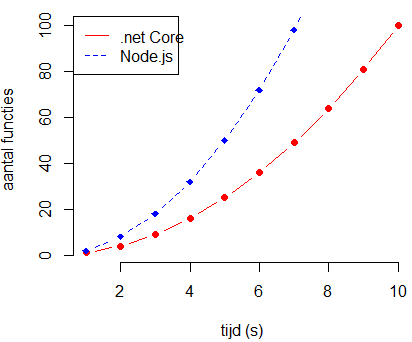
\includegraphics[width=8cm]{tijd_functies}

%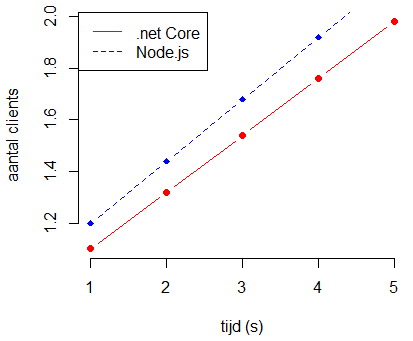
\includegraphics[width=8cm]{tijd_clients}

%---------- Verwachte conclusies ----------------------------------------------
\section{Verwachte conclusies}
\label{sec:verwachte_conclusies}
Uit dit onderzoek moet blijken dat één van de twee talen duidelijk sneller is. Het onderzoek zal niet in een echte omgeving uitgevoerd worden dus enkele statistieken kunnen over het hoofd gezien worden. Hopelijk vloeit uit dit onderzoek een duidelijke basis van vergelijking tussen Node en .net en bied het nieuwsgierige bedrijven nuttige informatie.